\documentclass[12pt, a4paper]{article}
\usepackage[ngerman]{babel}
\usepackage{graphicx}
\usepackage{wrapfig}
\usepackage{titlesec}
\usepackage{geometry}
\usepackage[font=scriptsize]{caption}
\usepackage{blindtext}
\usepackage{hyperref}
\usepackage{tabularx}
\usepackage[bottom]{footmisc}

\captionsetup{justification=raggedright,singlelinecheck=false}
\geometry{
  a4paper,% redundant if already in \documentclass
  left=25mm,
  right=25mm,
  top=25mm,
  bottom=25mm,
  heightrounded,% better use it
 }
 \titleformat{\chapter}[display]
   {\normalfont\bfseries}{}{0pt}{\huge}
  
\usepackage{lipsum}  
\graphicspath{ {./pics/} }
\author{Oleksii Baida}
\date{Novemver 2023}
\begin{document}
%\include{titelseite}

\tableofcontents
\pagebreak

\section{Einführung in IoT}
\par Das Ziel des IoT ist die Verbindung der physischen und digitalen Welt. Diese Verbindung besitzt großes Potential in verschiedenen Bereichen wie Logistik, Agrarwirtschaft, Smart Cities oder Gesundheitswesen. Das IoT befasst sich dabei mit der Vernetzung von Geräten und der Kommunikation zwischen allen Knoten. Durch die Vernetzung können die Endgeräte im Netzwerk selbstständig Daten sammeln, austauschen und an das Netzwerk senden. Auf Basis der gesammelten Daten kann das System Entscheidungen ohne menschliches Eingreifen treffen und auf bestimmte Ereignisse reagieren. 
\par Das Internet of Things (IoT)-System besteht aus fünf Komponenten: Se nsoren, Aktoren, Verbindungen, Datenverarbeitung und Benutzeroberfläche. Dadurch ergeben sich vier Software-Schichten des IoT-Systems: die Geräte-Schicht, die Kommunikationsschicht, die Cloud-Schicht und die Anwendungsschicht.
\par Sensoren und Aktoren gehören zur Geräte-Schicht. Sensoren erfassen kontinuierlich Daten aus der physischen Welt und übermitteln sie an das Netzwerk. Unter den Sensoren finden sich beispielsweise Temperatur-, Licht- und Bewegungssensoren. Über die Aktoren wirkt sich das IoT-System auf die physische Welt aus. Zu den Aktoren zählen Thermostate, Klimaanlagen, Lichtschalter und Servomotoren. 
\par Durch die Vernetzung werden die Sensordaten an einer zentralen Stelle gesammelt. Dies kann beispielsweise ein Mikrocontroller oder ein Server sein. Die Daten werden auf Basis objektiver Evaluierungen verarbeitet, damit Entscheidungen getroffen werden können. Sie werden hauptsächlich auf einem Server in der Cloud gespeichert und verarbeitet. Dies erleichtert die Steuerung des Systems und verbessert die Benutzerfreundlichkeit. Die Cloud ermöglicht es, die Daten an Anwendungen weltweit zu senden, um Systemzugriff überall zu ermöglichen. Beispiele für solche Systeme sind AWS IoT, NodeRED und Cisco IoT Cloud Connect.
\par Durch die Vernetzung der Endgeräte entsteht ein Netzwerk, das die Bereitstellung von Echtzeitdaten und die Automatisierung ermöglicht. Alle Geräte im System müssen mit dem Netzwerk verbunden und über das Netzwerk erreichbar sein. Alle Daten, die an das Netzwerk gesendet werden, müssen über die Zentrale laufen. Es ist wünschenswert, die Geräte drahtlos miteinander zu verbinden. Hierfür wurden verschiedene Protokolle wie KNX, MQTT oder Zigbee entwickelt. Diese ermöglichen den Austausch kleiner Datenmengen und reduzieren gleichzeitig den Stromverbrauch.
\par Durch die drahtlose Verbindung von physischer und digitaler Welt modernisiert das IoT verschiedene Branchen. Es vereinfacht die Logistik, indem es die Verfolgung von Gütern in Echtzeit ermöglicht. Es ermöglicht auch effizientere Energiesysteme, die Ressourcen sparen. Es gibt bereits viele Geräte für das Smart Home, die unseren Alltag vereinfachen. Auch in der Medizin wird das IoT breit genutzt. Spezielle tragbare Geräte ermöglichen es, den Gesundheitszustand von Patienten zu überwachen. Die Smartwatch unterstützt den Träger im Alltag, indem sie Gesundheitsempfehlungen gibt und die täglichen Aktivitäten aufzeichnet. 
\par Die Hauptvorteile des IoT sind die Bereitstellung von Echtzeitdaten, die Automatisierung von Steuerungssystemen und die drahtlose Vernetzung von Endgeräten. Zusammen bilden sie ein skalierbares und sicheres System, das relativ einfach eingerichtet und verwaltet werden kann. Es gibt auch viele Plattformen, die gut für die Entwicklung und das Testen von IoT-Systemen geeignet sind. Dazu gehören Arduino, Raspberry Pi, ESP32 usw. Mit diesen Plattformen kann man das Testsystem praktisch aufbauen, testen und dann das System für die reale Welt skalieren.
\pagebreak

\section{IoT Software Layers}

\subsection{Device-Layer (Geräte-Schicht)}
\par Zu der Geräte-Schicht gehören Sensoren, Aktoren und Controller Als Sensoren werden alle Geräte in einem IoT-System bezeichnet, die für die Erfassung relevanter Daten verwendet werden. Die Sensoren dienen als neutrale Überwachter der Arbeitsumgebung und haben keinen Einfluss auf die Umwelt. Die Sensoren erfassen eine breite Palette von Umweltparametern, wie Temperatur, Feuchtigkeit, Vibrationen oder Lärm. Sie erkennen Bewegungen im Raum und identifizieren Gase in der Luft. 
\par Die gesammelten Daten werden in das Netzwerk übertragen, wodurch physische Objekte zu datengenerierenden "Dingen" innerhalb des IoT-Ökosystems werden. In verschiedenen Systemen werden unterschiedliche Sensoren eingesetzt. Zum Beispiel für die Landwirtschaft wurden spezielle Sensoren eingesetzt, um physische Eigenschaften des Bodens und die Umweltbedingungen zu erfassen. In Smart-Home Systemen werden Sensoren eingesetzt, um die Temperatur in der Wohnung zu messen sowie Feuer, Rauch oder Bewegungen zu erkennen. Diese Sensoren sammeln nicht nur Daten, sondern übermitteln sie auch an die Zentrale, was eine intelligente und effiziente Interaktion zwischen physischen und digitalen Werten ermöglicht.
\par Aktoren sind die Geräte im IoT-System, die digitalen Befehle in physischen Aktionen umsetzen. Sie dienen als Brücke zwischen der digitalen Welt der Daten und physischen Welt der Aktionen. Sie wandeln digitale Signale in physische Bewegungen oder andere Aktionen um. Die Befehle werden durch Analyse von Daten von Controller erzeugt. Aktoren haben immer Einfluss auf die Arbeitsumgebung. Die Entscheidungen, die der Controller trifft, werden über die Aktoren in Aktionen umgesetzt. In Smart-Home-Systemen können Aktoren beispielsweise verwendet werden, um Heizungssysteme basierend auf Temperaturdaten zu regulieren oder Beleuchtung automatisch anzupassen. In industriellen Anwendungen ermöglichen Aktoren eine präzise Steuerung von Maschinen, was die Arbeit effizienter und sicherer macht. 
\par Der Controller hat eine wichtige Rolle in einem IoT-System. Er ist verantwortlich für die Verarbeitung und Interpretation der von den Sensoren gesammelten Daten. Der Controller sammelt alle Daten und analysiert sie, um intelligente Entscheidungen zu treffen. Je nach seiner Datenverarbeitungskapazität kann er die Aufgaben unterschiedlicher Schwierigkeitsgrade koordinieren. Außerdem reagiert er auf dynamische Änderungen der Umgebungsbedingungen. Es ermöglicht dem Controller, präzise Befehle an Aktoren zu senden, um verschiedene automatisierte Aktionen auszuführen. Ein Beispiel dafür ist das Ein- oder Ausschalten der Klimaanlage bei einer Änderung der Temperatur.

\subsection{Kommunikation-Layer (Kommunikationsschicht)}
\par Die Kommunikationsschicht bezeichnet die Verbindungen zwischen allen Komponenten eines IoT-Systems. Hier werden Protokolle und Standards für eine sichere, zuverlässige und reibungslose Kommunikation zwischen den Geräten im System definiert. Die Verbindung erfolgt über verschiedene Protokolle wie MQTT, KNX oder XMPP. Mehr zu KNX und MQTT weiter unten.
\subsubsection{KNX}
\par KNX ist ein öffentlicher Standard für die Gebäudeautomatisierung. Es ermöglicht sowohl eine drahtgebundene Verbindung über verdrillte Zweidrahtleitung oder Ethernet als auch eine drahtlose Verbindung über Funk (KNX-RF) mittels KNX-Transceiver. KNX-RF ist eine drahtlose Variante des KNX-Protokolls. Es eignet sich gut für die Automatisierung von Gebäuden und kann auch mit anderen drahtlosen IoT-Protokollen wie Zigbee oder Z-Wave kombiniert werden. Das KNX-Protokoll bietet eine bequeme Benutzeroberfläche zur Einstellung und Steuerung des Systems.
\par Der größte Vorteil von KNX ist, dass keine zentrale Steuerung benötigt wird. Jedes Gerät im System verfügt über einen eigenen Mikroprozessor und die Fähigkeit, Daten zu analysieren. Die Sensoren senden Befehle in Form eines Telegramms direkt an Aktoren, ohne dass die Daten über eine zentrale Stelle laufen müssen. Dadurch ist es möglich, Geräte unterschiedlicher Hersteller zu verbinden, die das KNX-Protokoll unterstützen. Es gibt eine große Auswahl an Geräten mit KNX-Protokoll auf dem Markt.
\subsubsection{MQTT}
\par Das MQTT-Protokoll\footnote[1]{Message Queuing Telemetry Transport} ist ein einfaches, effizientes und leichtgewichtiges Nachrichtenprotokoll, das speziell für den Einsatz in IoT-Systemen entwickelt wurde. Es ermöglicht die Kommunikation von Geräten mit geringer Bandbreite und begrenzten Ressourcen. Das Protokoll basiert auf dem Publish-Subscribe-Modell und erfordert daher eine zentrale Instanz, den Broker. Dies ermöglicht es den Geräten, Nachrichten an einen zentralen MQTT-Broker zu senden und von diesem zu empfangen. Die Nachrichten werden unter Topics veröffentlicht, welche Kanäle darstellen, zu denen sich Subscriber registrieren können. Das Backend für das MQTT-Protokoll kann mit NodeRed realisiert werden. NodeRed bietet ein sehr benutzerfreundliches Interface, um die Nachrichten vom Publisher zu empfangen, zu verarbeiten und an ein Endgerät zu senden, wie zum Beispiel einen Telegram-Bot oder ein Cloud-System.
\par MQTT wird aufgrund seiner Unkompliziertheit oft in Smart-Home-Anwendungen verwendet. Es zeichnet sich durch eine gute Zuverlässigkeit aus, da die Nachrichten immer in einer bestimmten Reihenfolge vermittelt werden. Jede Nachricht wird genau einmal gesendet. Obwohl es keine Garantie für die Zustellung der Nachricht gibt, werden Duplikate vermieden. MQTT ermöglicht das Speichern der letzten Nachricht im Topic, wodurch neue Abonnenten diese Nachricht sofort nach der Registrierung zum Topic erhalten. Aus eigener Erfahrung kann ich bestätigen, dass es bei häufigem Senden der Nachrichten keine Probleme mit der Zustellung gibt. Wenn Nachrichten für eine bestimmte Zeit ausbleiben, sollte überprüft werden, ob die Verbindung unterbrochen ist. MQTT bietet Last-Will-und-Testament-Funktion, was ermöglicht dem Broker eine bestimmte Nachricht bei dem Ausfall der Verbindung zu senden. Diese Nachricht kann bei der Registrierung des Subscribers zum Topic definiert werden und wird im Brocker gespeichert, bis er einen Verbindungsausfall erkennt.ß
\par Bei der Wahl des Protokolls sollten die Entwickler die folgenden Schlüsselpunkte berücksichtigen:
\begin{itemize}
  \item[\textbullet] \textbf{Data latency} – Wie schnell sollen die Daten übergeben werden? Wie kann man ein Packet vom Startpunkt zum Endpunkt vernünftig übergeben?
  \item[\textbullet] \textbf{Reliability} – Welche Folgen hat Datenverlust im IoT-System? Wie kann das System zuverlässiger werden?
  \item[\textbullet] \textbf{Bandwidth} – Wie groß sind Datenmengen, die transportiert werden sollen?
  \item[\textbullet] \textbf{Transport} – Welches Protokoll ist für den Transport am besten geeignet? Am meisten wird zwischen TCP, UDP und http entschieden.
\end{itemize}

\subsection{Cloud-Layer (Cloud-Schicht)}
\par Die Cloud-Schicht ist der Ort, an dem die gesammelten Daten gespeichert, verarbeitet und analysiert werden. Diese Schicht umfasst die Backend-Infrastruktur, wie zum Beispiel Server, Datenbanken, Speicher und Analysetools. Durch diese zentrale Plattform wird eine hohe Skalierbarkeit und Flexibilität des Systems ermöglicht, sodass die Verwaltung großer Datenmengen vereinfacht wird. Sicherheitsmaßnahmen werden ebenfalls in dieser Schicht implementiert, um die Daten vor unautorisiertem Zugriff zu schützen. Abstriche werden dabei nicht gemacht.
\subsubsection{AWS IoT}
\par Amazon Web Services bietet eine Cloud-Plattform, die IoT-Geräte mit Cloud-Diensten verbindet. Sie ermöglicht die sichere Verbindung von Geräten und die Verarbeitung und Speicherung von Daten direkt in der Cloud. Auch besonders große Datenmengen, wie beispielsweise beim autonomen Fahren gesammelt werden, können in der Cloud verarbeitet und gespeichert werden. Es unterstützt verschiedene Kommunikationsprotokolle und Ende-zu-Ende-Verschlüsselung.
\par Auf AWS IoT können Anwendungen unterschiedlicher Komplexität laufen. Es können sowohl große industrielle Systeme als auch kleinere Systeme für die Haussicherheit oder Ähnliches laufen. Zu den Kunden gehören auch große Konzerne. So nutzt beispielsweise Volkswagen AWS IoT, um die Effizienz und Verfügbarkeit seiner Anlagen zu erhöhen und die Qualität seiner Fahrzeuge zu verbessern.
\subsubsection{Cisco IoT Cloud Connect}
\par Die von Cisco angebotene Plattform für IoT-Systeme wurde speziell für Mobilfunkbetreiber entwickelt. Sie bietet Optimierung, Sicherheit und Flexibilität für das Management von IoT-Verbindungen. Die Plattform unterstützt Mobilfunkbetreiber bei der effizienten Verwaltung ihrer IoT-Dienste. Außerdem ermöglicht sie eine bessere Kontrolle über die Konnektivität, die Datennutzung und die Sicherheit der angeschlossenen Geräte. Cisco bietet auch ein Kontrollzentrum an, in dem die IoT-Systeme konfiguriert werden können. Eine Besonderheit ist die Erkennung von Anomalien bei Geräten oder Verbindungen, die mit Hilfe von KI funktioniert. Insgesamt ist Cisco IoT Cloud Connect eine innovative und effiziente Plattform, die sich sehr gut für große IoT-Systeme eignet.
\subsubsection{Google Cloud IoT}
\par Die Google-Plattform bietet eine umfassende Lösung für Gerätemanagement, Datenverarbeitung und maschinelles Lernen direkt in der Cloud. Die Plattform ist eine Reihe von Cloud Computing-Diensten. Google Cloud IoT läuft auf derselben Plattform, die Google auch für andere Dienste wie YouTube oder Google Search verwendet. IoT-Geräte können drahtlos mit der Plattform verbunden werden. Von Google entwickelte Dienste für künstliche Intelligenz oder maschinelles Lernen können genutzt werden. 
\par Google Cloud IoT Core ist Bestandteil der Plattform. Es hat einen großen Vorteil, da es einen automatischen Lastausgleich und eine Datenskalierung bietet. Das Core besteht aus zwei Hauptkomponenten: Device Manager und Protocol Bridge. Device Manager hilft bei der Registrierung der Geräte bei den Diensten und stellt auch den Mechanismus für die Authentifizierung der Geräte bereit. Er verwaltet auch eine logische Konfiguration für jedes Gerät und kann für die Fernsteuerung des Geräts über die Cloud verwendet werden. Protocol Bridge bietet eine Möglichkeit für die Geräte, auf die Google Cloud zuzugreifen oder sich mit einigen Standardprotokollen wie HTTP und MQTT zu verbinden. Dies ermöglicht es den Entwickler, ihren bestehenden Geräten mit minimalen Änderungen an der Firmware zu verwenden. Die von Google entwickelte Plattform bietet außerdem eine benutzerfreundliche Schnittstelle für Entwickler. In meiner Projektarbeit plane ich, die Plattform besser kennenzulernen und anzuwenden.

\subsection{Application-Layer (Anwendungsschicht)}
\par Die Anwendungsschicht stellt die Dienste des IoT-Systems für die Nutzer bereit. Sie basiert meist auf der Cloud und stellt die verarbeiteten Daten in einer Benutzerschnittstelle dar. Über die Anwendungsschicht interagieren die Nutzer mit dem System. Es ist wichtig, dass die Anwendungsschicht die unterschiedlichen Bedürfnisse und Erwartungen der verschiedenen Benutzer erfüllt.
\par Die Anwendungsschicht ist die wichtigste Schicht für die Nutzer eines IoT-Systems. Sie muss eine intuitive und benutzerfreundliche Schnittstelle bieten, die die Daten klar und verständlich darstellt. Die Schnittstelle kann je nach Anwendungsfall unterschiedlich gestaltet werden. Die Benutzer können den Zustand des Systems und die Sensordaten einsehen sowie Befehle an das System senden. Dazu werden verschiedene Protokolle wie MQTT, CoAP oder REST verwendet. Die Wahl des Protokolls hängt von der Datenmenge und den Netzwerkbedingungen ab.
\par Die Anwendungsschicht bietet auch die Möglichkeit, die Daten des IoT-Systems mit anderen Diensten zu integrieren. Beispielsweise können die Daten an Online-Dienste oder Sprachassistenten weitergeleitet werden. Dies erweitert die Funktionalität und Interaktivität des Systems und ermöglicht eine personalisierte Benutzererfahrung. Die Integration kann über verschiedene APIs erfolgen, die von den Cloud-Plattformen zur Verfügung gestellt werden. Die Anwendungsschicht kann auch maschinelles Lernen oder künstliche Intelligenz nutzen, um Daten zu analysieren und Muster oder Anomalien zu erkennen. Dies kann zu einer besseren Optimierung und Vorhersage des Systemverhaltens führen.
\par Die Anwendungsschicht muss ein hohes Sicherheitsniveau aufweisen, da sie die Schnittstelle zum Benutzer und zu den Endgeräten darstellt. Wenn es eine Sicherheitslücke in der Anwendungsschicht gibt, ist das gesamte System gefährdet. Die Architektur der Anwendungsschicht hat kritische Auswirkungen auf die Effizienz und Funktionalität des gesamten Systems. Daher muss diese Schicht bewusst auf die Anforderungen der Systemkomponenten ausgelegt werden. Die oben beschriebenen Cloud-Plattformen bieten die Bereitstellung der Daten für die Nutzer, d.h. die Anwendungsschicht wird direkt in der Cloud implementiert. Dies hat große Vorteile, da die Sicherheit der Schicht durch die Nutzung der Cloud-Dienste aufgebaut wird. Darüber hinaus kann die Ausgabe der Daten für alle Nutzer gleichzeitig komfortabel in der Cloud konfiguriert werden.
\pagebreak

\section{Matter}
\par Das Matter-Protokoll ist ein neues Protokoll für IoT-Systeme. Es wurde im November 2022 von CSA\footnote[2]{Connectivity Standards Alliance} eingeführt. Das Hauptziel des Protokolls ist die Verbesserung der Interoperabilität und Kompatibilität zwischen Geräten unterschiedlicher Hersteller sowie die Erhöhung der Sicherheit. Es erlaubt die Interaktion zwischen verschiedenen Geräten, Protokollen und Verbindungen und erleichtert somit die Integration von Matter-Geräten in ein IoT-System. Matter-Protokoll ist ein Open-Source-Standard. Matter nutzt die Leistungsfähigkeit von IPv6 und UDP\footnote[3]{User Datagram Protocol}. Es wurde vom Project Connected Home Over IP entwickelt und wird derzeit von CSA verwaltet. 

\subsection{Eigenschaften}
\begin{description}
  \item [Hohe Sicherheit:] Die Sicherheit des Matter-Protokolls hat mehrere Schichten. Es setzt eine Vielzahl von Sciherheitsmethoden, wie AES\footnote[4]{Advanced Encryption Standard} und CCM\footnote[5]{Cloud Controls Matrix}. Außerdem erlaubt das Protokoll die Datenintegrität durch SHA-256. Die wesentlichen Merkmale von Matter im Bereich Sicherheit sind die Protokolle Zero Trust und Security by Design. Zero Trust stellt sicher, dass nur die authentifizierten Benutzer auf die Daten zugreifen können. Security by Design zielt darauf ab, Systeme durch kontinuierliche Tests und die Einhaltung idealer Programmiermethoden frei von Schwachstellen und Angriffen zu halten.
  \item [Offline IoT Computing:] An der Geräte-Schicht verwendet Matter ein Thread-Protokoll. Thread ist ein drahtloses, energieeffizientes Mesh-Protokoll, das es verbundenen Geräten ermöglicht, ohne eine zentrale Stelle miteinander zu kommunizieren. Es erlaubt die Verarbeitung der Daten offline. Mit der Fähigkeit zur direkten Kommunikation untereinander benötigen die Geräte keinen Internetzugang. Diese Eigenschaft von Matter macht es besonders sicher für Geräte wie Sicherheitskameras und intelligente Schlösser. 
  \item [Energieeffizienz:] Durch die Anwendung des Thread-Protokolls weist Matter eine sehr gute Energieeffizienz auf. Geräte, die über Thread kommunizieren, verbrauchen beim Datenaustausch wenig Strom und die Frequenz der Datenübertragung ist ebenfalls gering. Wenn keine Daten übertragen werden müssen, schalten sich die Geräte aus, was zu einer erheblichen Ersparnis an Strom führt.
  \item [Datenschutz:]Matter verarbeitet die Benutzerdaten nicht direkt. Es verarbeitet Daten, die zu und von Geräten im Netzwerk fließen. Um sicherzustellen, dass Daten von oder zu registrierten Matter-Geräten fließen, muss jedes Gerät seine Identität nachweisen. Matter verwendet so wenig Daten wie möglich. Damit ist es einfacher die Daten zu sichern 
\end{description}

\subsection{Funktionsweise}
\par Matter liegt auf der Anwendungsschicht von TCP/IP. Es verwendet UDP und IPv6. Die Matter-Geräte in Smart Home-Systemen verwenden vor allem WiFi (Ethernet) und Thread. Die Verbindung mit dem Internet und der Cloud kann über zentrale Hubs wie Google Home oder Alexa erfolgen.
\par Das Thread-Protokoll verbindet Geräte mit geringer Bandbreite innerhalb des Systems. Zu diesen Geräten gehören Lampen, Sicherheitskameras, Smartschlösse, Feuermelder usw. Thread Border Router verbindet das Thread-Netzwerk mit dem globalen Netzwerk. Jedes Thread-Gerät kann ein Router werden, da die Daten zwischen den Knoten an der Zentrale durch Hopping übermittelt werden. Dadurch wird eine sogenannte Selbstheilung ermöglicht. Selbstheilung bedeutet, dass im Falle eines Knotenausfalls die Daten automatisch über einen anderen Knoten übermittelt werden.
\par IIn Matter gibt es keine vertikale Hierarchie. Controller und Controlee stehen auf der gleichen Ebene. Aber jedes Gerät ist nach Device Data Model hierarchisch aufgebaut.


\subsection{Device Data Model}
\subsubsection{Device Types}
\par Gemäß der Spezifikation des Matter-Protokolls muss jedes Gerät ein oder mehrere Device Types implementieren oder erweitern. Die Device Types sind nicht direkt in der Matter-Dokumentation definiert, sondern in einem anderen Dokument namens 'Device Library' von CSA. Eine Anfrage zur Dokumentation kann unter folgendem Link\footnote[6]{https://csa-iot.org/developer-resource/specifications-download-request/} gestellt werden. Beispiele für Device Types sind 'Door Lock', 'Video Player' und 'On/Off Switch'.
\subsubsection{Nodes}
\par Alle Geräte im System sind als Knoten bezeichnet. Die Knoten sind eindeutig identifizierbar und stehen dem Benutzer im Netzwerk zur Verfügung. Die Kommunikation in Matter findet zwischen diesen Knoten statt. Matter bietet 5 verschiedene Arten von Knoten (Node Roles):
\begin{description} 
  \item [Commissioner:] Commissioner in Matter hinzufügt neue Geräte ins System und übergibt denen nötige Daten.
  \item [Controller:] Ein Knoten, der ein oder mehreren Knoten kontrolliert. Nicht jedes Gerät kann ein Controller sein, aber viele Controller können gleichzeitig Controlee werden.
  \item [Controlee:] Ein Knoten, der von einem oder mehreren Controllern gesteuert ist. Manche Geräte können nur Controlee sein (Lichtbirne), andere aber nur Controller (On/Off Switch).
  \item [OTA Provider:] OTA\footnote[7]{Over-The-Air} Ein Knoten, der Softwareaktualisierungen zur Verfügung stellt.
  \item [OTA Requestor:] Ein Knoten, der die Softwareaktualisierungen anfragt.
\end{description}

\subsubsection{Endpoints}
\begin{wrapfigure}{r}{0.4\textwidth}
  \centering
  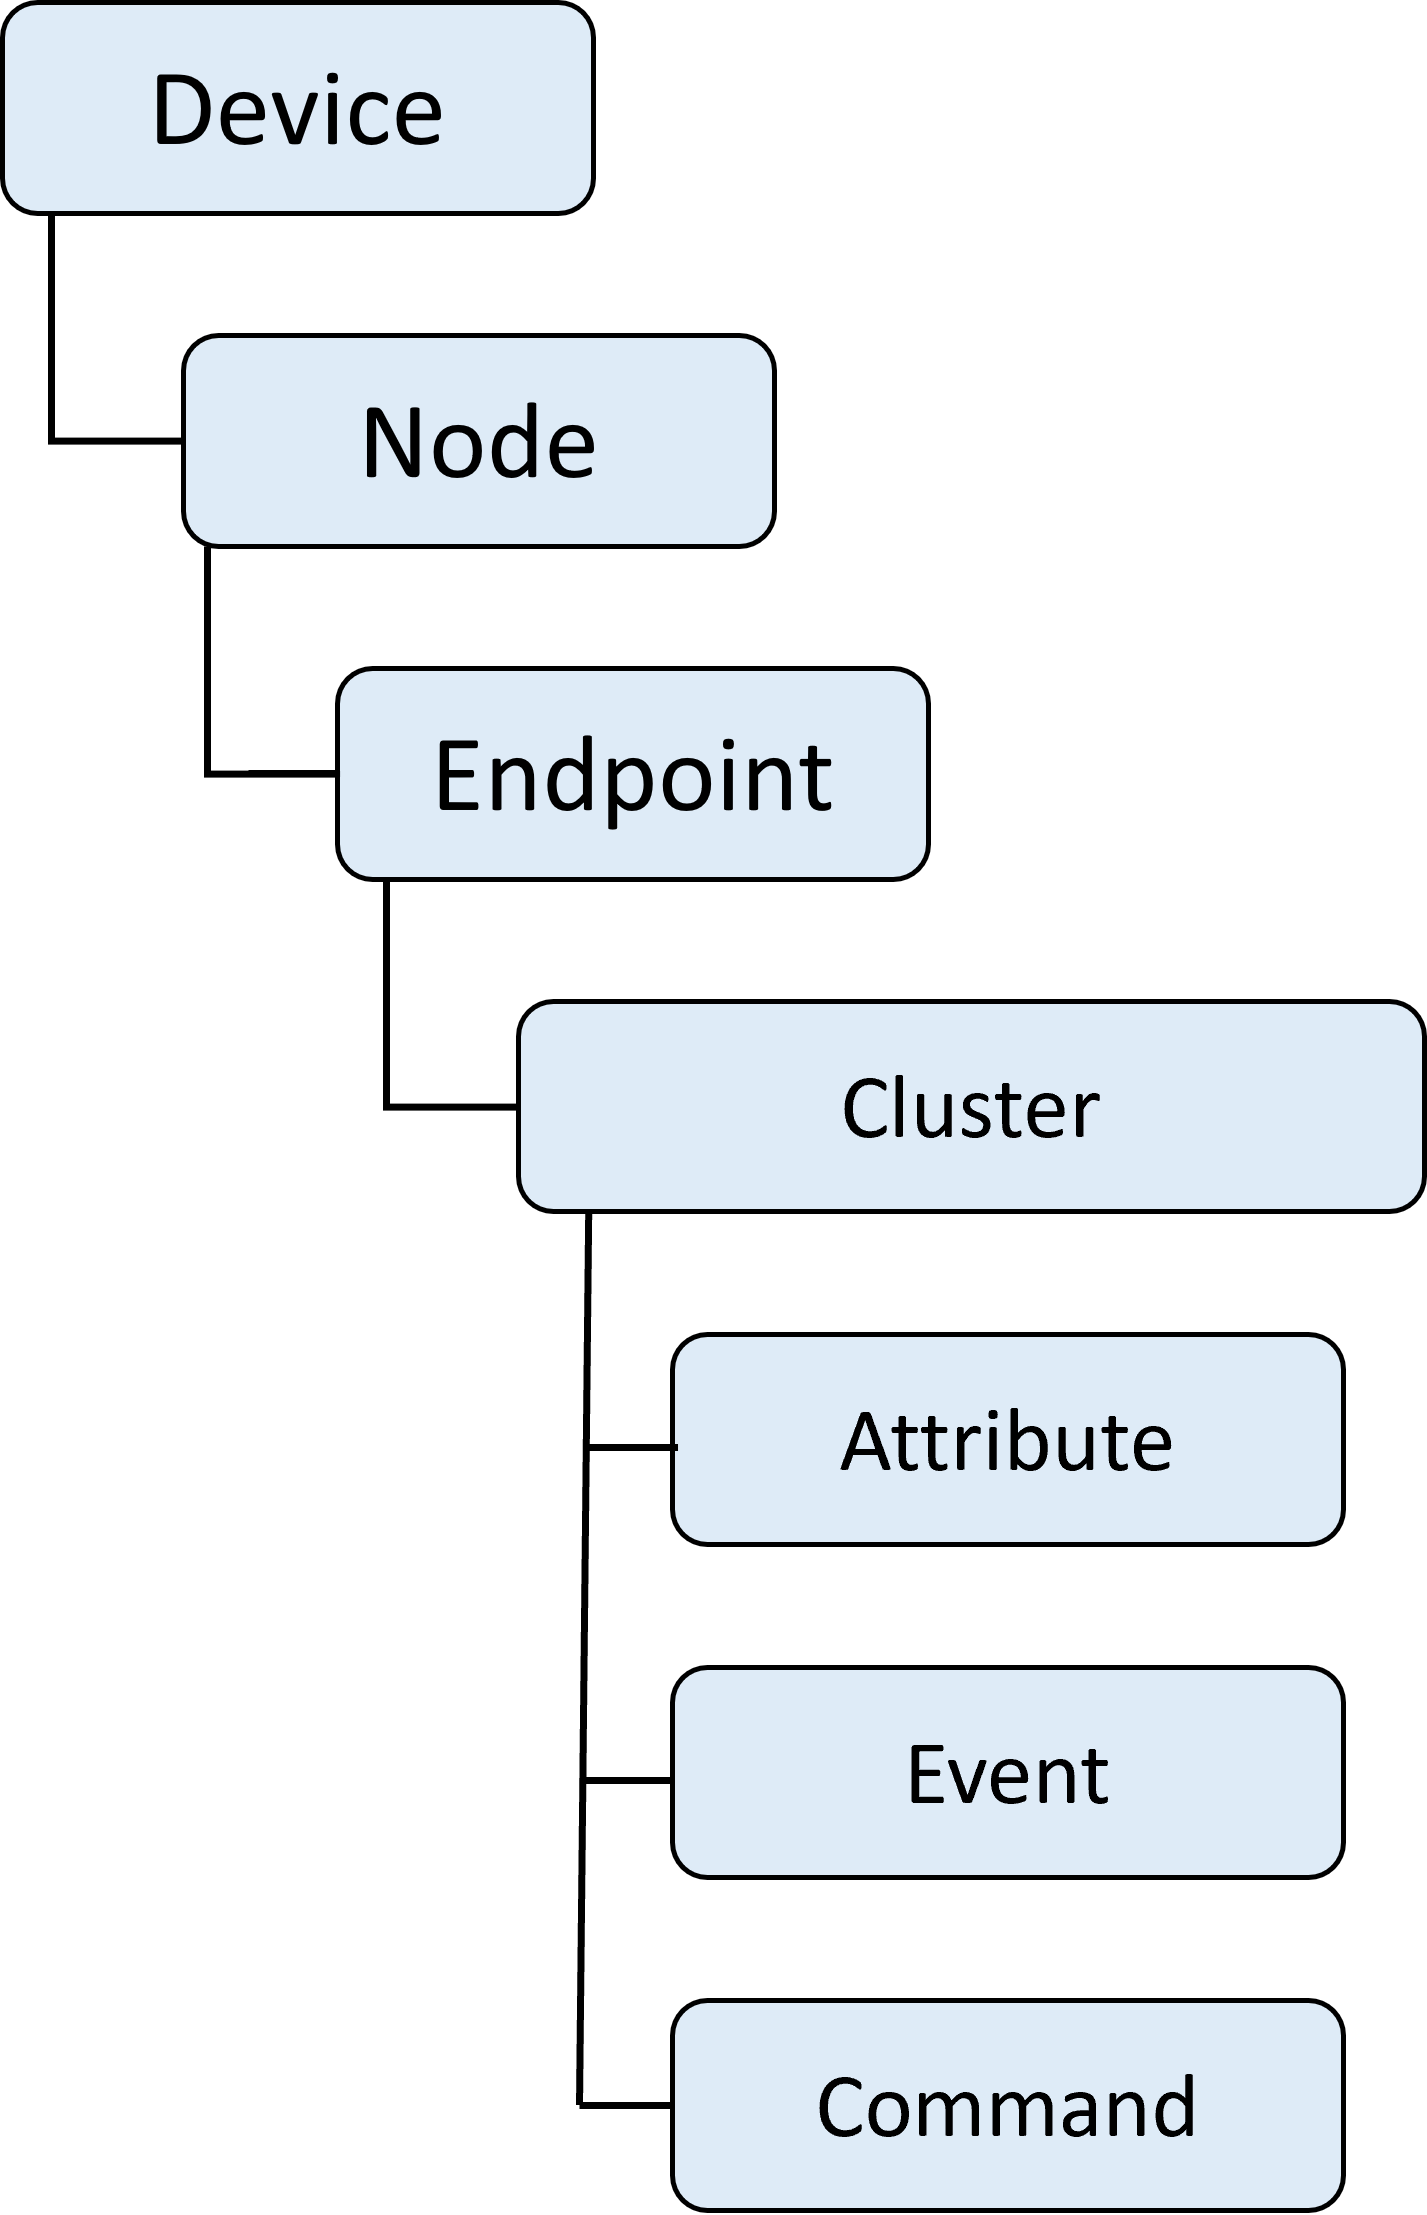
\includegraphics[scale=0.5]{ddm}
  \caption{Matter Device Data Model}
  \label{Matter Device Data Model}
\end{wrapfigure}
\par Jeder Knoten soll eine oder mehrere Funktionen ausführen. Diese Funktionen sind in Endpoints verfasst. Jedes Endpoint definiert eine Funktion, die das Gerät ausführen kann. Einige Geräte können verschiedene Funktionen ausführen, wie beispielsweise Smartphones oder Klimaanlagen. Deshalb kann ein Knoten aus mehreren Endpoints bestehen. 
\subsubsection{Commands und Events}
\par Commands sind in Clustern gespeichert. Commands sind Aktionen, die das Gerät ausführen kann. Sie sind in normaler Sprache definiert. Zum Beispiel Command „turn off“ für „On/Off Switch“. Commands können Antworten und Ergebnisse erzeugen. In Matter sind solche Antworten auch als Commands definiert, die zwar in Gegenrichtung gehen.
\par Events sind auch in Clustern gespeichert. Während Attributes den aktuellen Zustand speichern, speichern die Events die vergangenen Zustände. Events enthalten monot steigende Zähler, sowie Zeitstempel und Priorität. Sie ermöglichen die Erfassung von Zustandsübergängen und eine Datenmodellierung, die mit Attributen allein nicht möglich ist.
\subsubsection{Cluster und Attributes}
\par Im Knoten befindet sich das Cluster eine Ebene unterhalb des Endpunkts. Der Endpunkt enthält ein oder mehrere Cluster, welche spezifische Informationen wie Geräteinformationen, Geräteeinstellungen und Funktionsbeschreibungen gruppieren. Diese Informationen sind in Attributen gespeichert.
\par Attributes liegen an der tiefsten Ebene in Device Hierarchie. Attributes speichern Zustand des Knotens, oder seine spezifische Information. 
\par Clusters können entweder Client-Cluster oder Server-Cluster sein. Server-Cluster sind stateful und speichern Attribute, Events und Commands. Client-Cluster sind hingegen stateless und leiten die Interaktionen mit dem Server ein. Sie lesen und ändern Attribute, lesen Events und rufen Commands auf. Ein Knoten kann gleichzeitig ein Server und ein Client sein, abhängig von den verschiedenen Clustern.
\par Einen anderen Typ von Cluster ist Descriptor Cluster.   Er beschreibt das Endpoint, einschließlich seiner Server- und Client-Cluster, Gerätetypen und anderer Endpunkte, nämlich Parts. Jeder Device Type benötigt ein Descriptor-Cluster. Das Root Device Type ist im Endpoint 0 definiert. Im Descriptor-Cluster sind alle relevanten Daten für Benutzer über das Gerät gespeichert. Der Commissioner und die Controlling Devices nutzen die Informationen im Descriptor Cluster, um das Gerät zu steuern und zu verwenden.

\subsection{Interaction  Model}
\par Das Interaktionsmodell des Matter-Protokolls definiert die Interaktionen zwischen den Data Models verschiedener Knoten. Im Matter gibt es drei Arten von Interaktionen: Lesen und Abonnieren von Attributen und Events, Schreiben von Attributen und Ausführen von Commands. Zwei Knoten können erst nach der Erstellung einer verschlüsselten Kommunikation zwischen sich kommunizieren. Interaktionen bestehen aus einem oder mehreren Transaktionen, die jeweils aus einer oder mehreren Aktionen bestehen. Die Knoten im Matter-Netzwerk können gruppiert werden, um das Senden und Empfangen von Daten zu und von mehreren Knoten gleichzeitig zu ermöglichen. Das erfolgt dann in einer Aktion. Jede Gruppe hat eine eindeutige 16-Bit-Gruppen-ID, die von allen Knoten in der Gruppe geteilt wird.
\par Der Knoten, der die Transaktion initiiert, wird Initiator genannt. Der zweite Knoten, der die Anweisungen erhält, wird Target genannt. In der Regel ist der Initiator der Client-Cluster und der Server-Cluster ist der Target. Es gibt zwei Arten von Transaktionen: Timed und Untimed. Timed Transaktionen haben ein maximales Zeitlimit für eine Lese- oder Schreibaktion. Das Zeitlimit soll Man-in-the-Middle-Angriffe auf das System verhindern. Timed Transaktionen werden meistens an die Knoten gesendet, die für die Bereitstellung des Zugriffs verantwortlich sind.
\par Bei der Ausführung jeder Transaktion muss der Path angegeben werden. Der Path definiert den Pfad zum Attribute, Event oder Command im Device Model des anderen Knotens. Der Pfad kann auch eine Gruppen-ID enthalten. Im Allgemeinen ist der Path wie folgt definiert:
\par \texttt{<path>} = \texttt{<node>} \texttt{<endpoint>} \texttt{<cluster>} \texttt{<attribute | event | command>}
\par \texttt{<path>} = \quad\quad\texttt{<group ID>}\quad\quad \texttt{<cluster>} \texttt{<attribute | event | command>}

\subsubsection{Read Transaktion}
\begin{figure}[h]
  \centering
  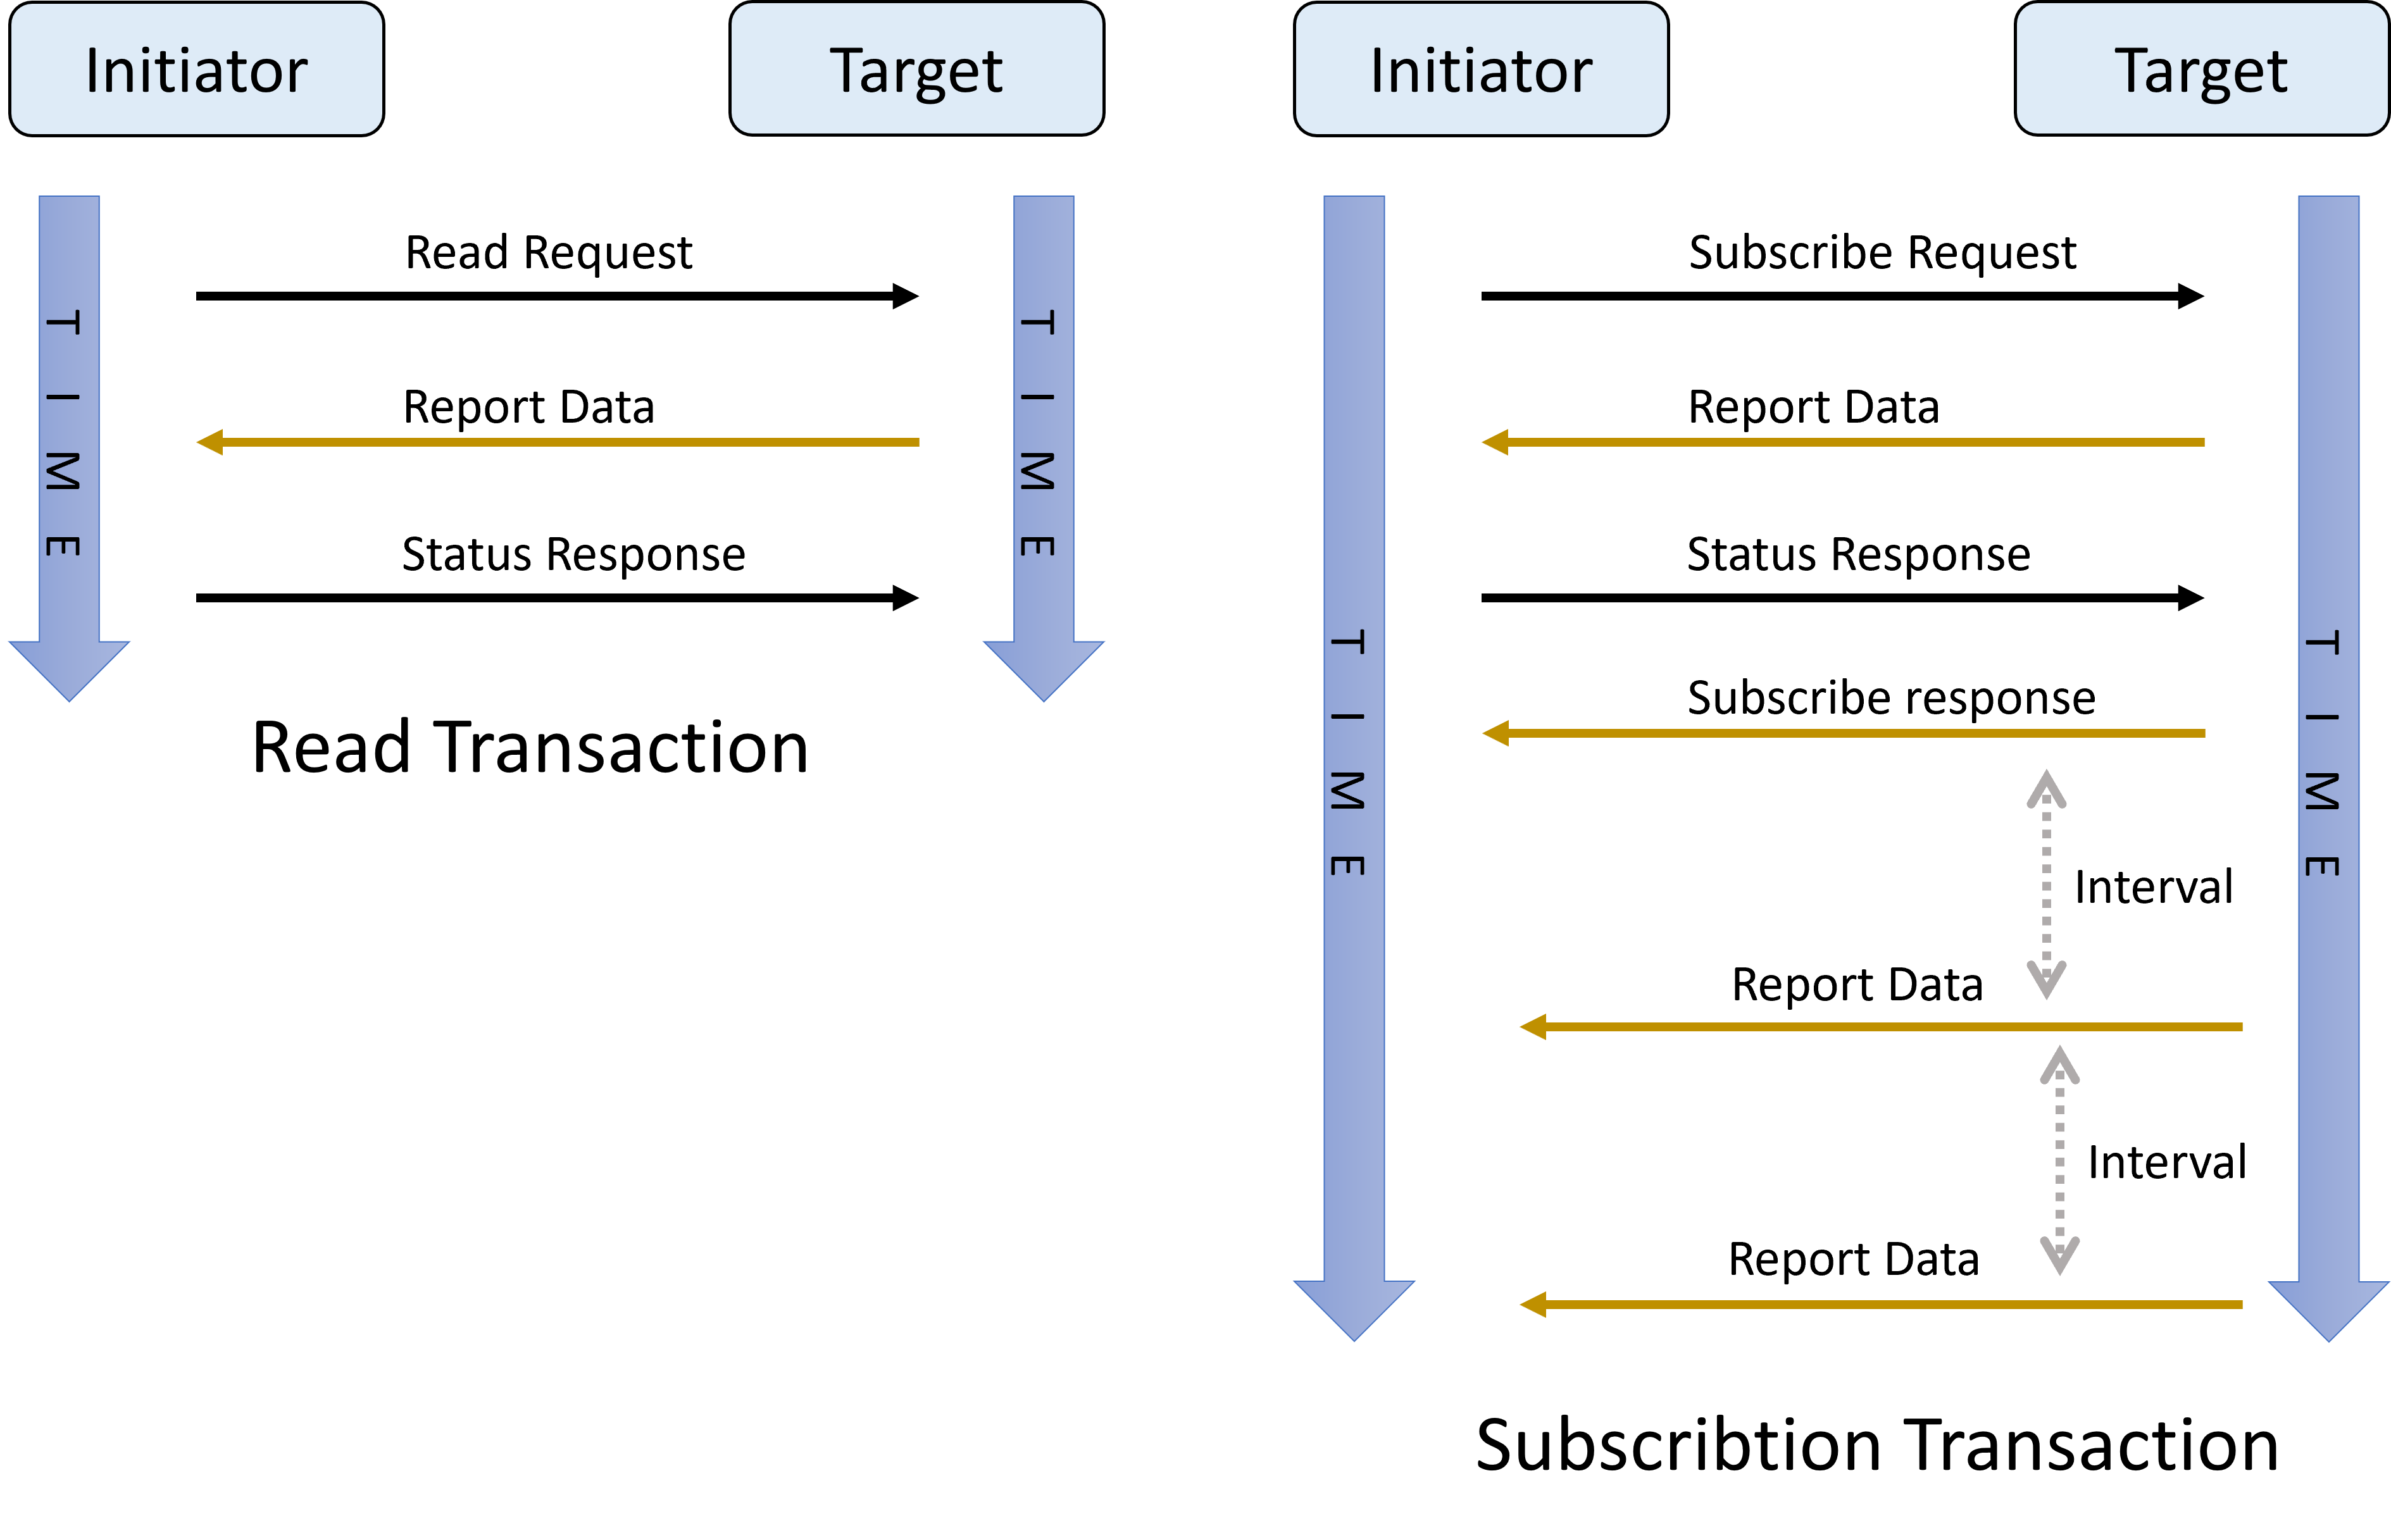
\includegraphics[scale=0.5]{read}
  \caption{Read and Subscription Transaction}
  \label{Read and Subscription Transaction}
\end{figure}
\par Die Read Transaction besteht aus drei Aktionen (siehe Abbildung 2). Zunächst fragt der Initiator die Liste der Pfade zu den angeforderten Attributen oder Events an (Read Request). Diese Aktion kann nur Unicast sein. Nach Erhalt der Anfrage stellt das Target eine Report Data Action zusammen.  Das Target kann mit vier Reports antworten: Attribute Report, Event Report, Suppress Response und Subscription ID. Das Flag 'Suppress Response' gibt an, ob das Status-Response benötigt wird. Bei der Anmeldung ist die Subscription ID erforderlich, um die Transaktion zu identifizieren. Die Status Response Action bestätigt den Erfolg der Transaktion oder sendet eine Fehlermeldung. Diese kann in beide Richtungen gehen. Wenn die angeforderten Daten empfangen werden, generiert der Initiator eine Status Response Action. Wenn das Flag 'Suppress Status Response' gesetzt ist, muss der Initiator die Aktion nicht senden.
\par In Matter bedeutet Subscription, dass der Initiator regelmäßig Daten vom Target erhält. Der Subscribe Request enthält das minimale und maximale Intervall zwischen den Reports sowie die Liste der Pfade zu den angeforderten Attributen oder Events. Der Target antwortet mit derselben Report Data Aktion wie bei der Lesetransaktion. Alle Report Data Aktionen müssen dieselbe Subscription ID haben. Die Subscribe Response Action geht vom Target zum Initiator. In dieser Aktion werden die Subscription ID sowie die minimalen und maximalen Intervalle übermittelt. Wenn der Subscriber innerhalb dieser Intervalle keine Antwort erhält, wird das Subscription storniert. Eine manuelle Stornierung ist ebenfalls möglich.

\subsubsection{Write Transaction}
\begin{figure}[h]
  \centering
  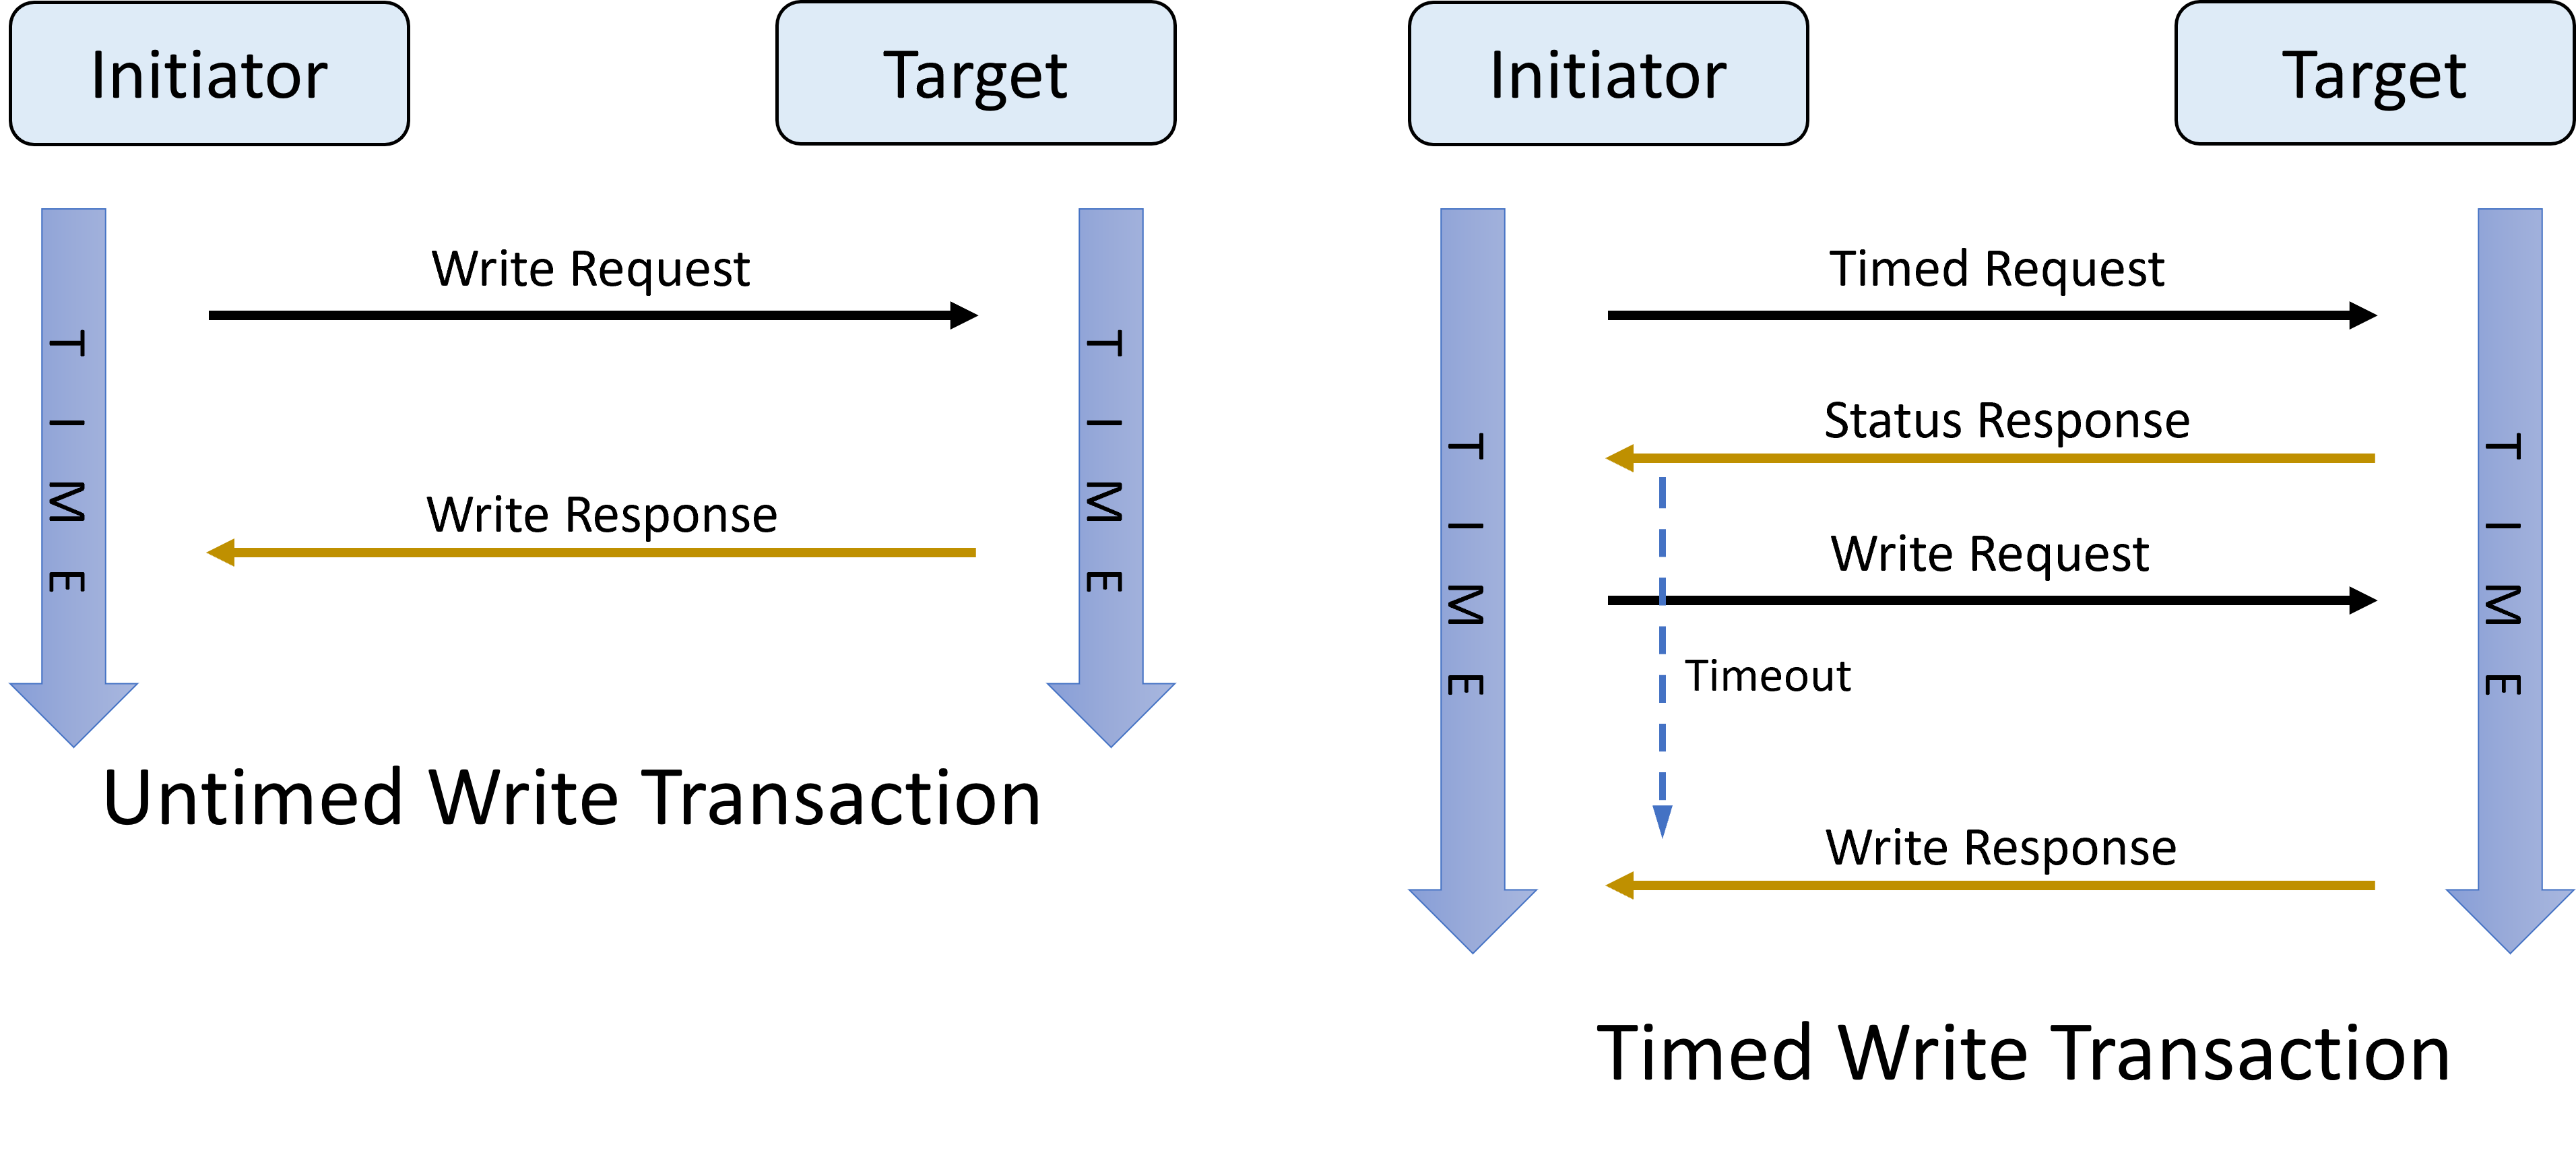
\includegraphics[scale=0.5]{write}
  \caption{Wrte Transaction}
  \label{Write Transaction}
\end{figure}
\par Die Write-Transaktion kann entweder als Timed oder Untimed ausgeführt werden. Bei einer Timed Transaction wird zuerst eine Timed Request gesendet und das Response wird erst nach einer Zeitüberschreitung (Timeout) in Millisekunden gesendet. Das Timed Request ist ein Flag, das die Art der Transaktion angibt. Der Write Request ist eine Liste von Daten und Pfaden zu den Elementen, die geändert werden sollen. Beim Groupcast muss das Flag Suppress Response gesetzt sein.  Der Write Response ist eine Liste von Pfaden und enthält auch Fehlermeldungen für jeden Write Request.

\subsubsection{Invoke Transaction}
\begin{figure}[h]
  \centering
  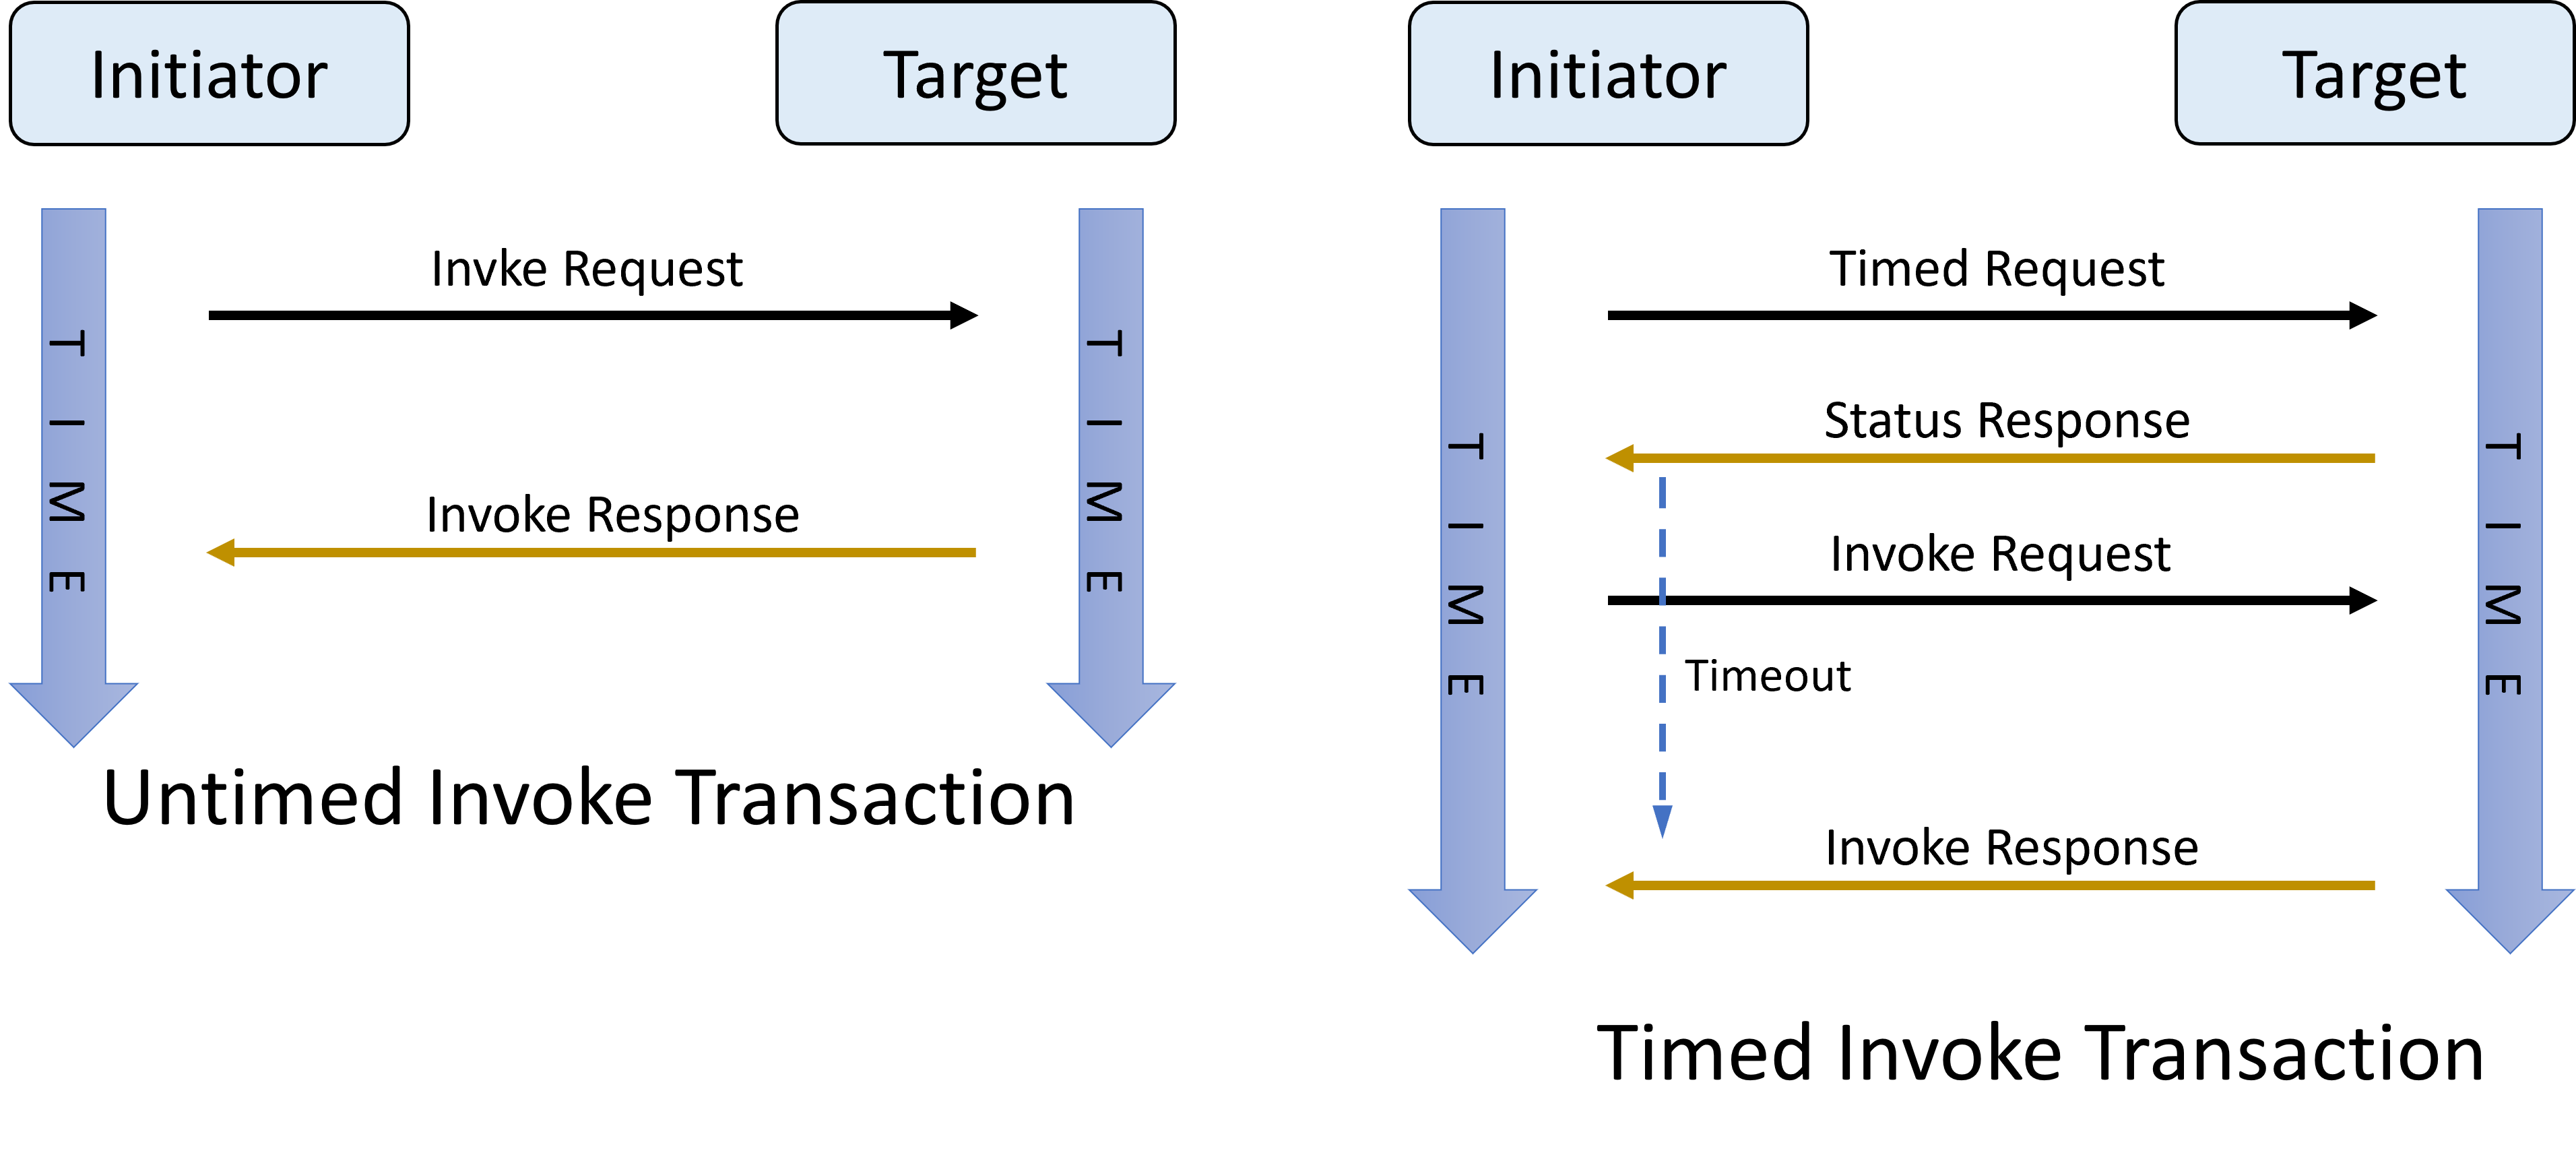
\includegraphics[scale=0.5]{invoke}
  \caption{Invoke Transaction}
  \label{Invoke Transaction}
\end{figure}
\par Die Invoke-Transaktionen sind für die Ausführung von Befehlen zuständig. Ähnlich wie bei den Write-Transaktionen gibt es Timed- und Untimed-Invoke-Transaktionen. Der Invoke-Request enthält eine Liste von Pfaden zu den Commands-Clustern und erforderlichen Argumenten für die Commands. Die Argumente werden als Command Fields bezeichnet. Interaction ID wird verwendet, um Requests an Responses anzupassen. Invoke Response enthält eine Liste der Responses der ausgeführten Kommandos und ggf. Fehlermeldungen. Wie bei der Write-Transaktion muss das Flag Suppress Response beim Groupcast gesetzt sein. Timed Request Action, Invoke Request Action und Invoke Response Action sind Unicast-only-Aktionen.

\subsubsection{Commissioning}
\par Das Commissioning im Matter-Protokoll ist ein Prozess, bei dem neuen Geräten Einstellungen zugewiesen werden. Dabei agiert ein oder mehrere Geräte als Commissioner. Das neue Gerät wird als Commissionee bezeichnet. Die Sequenz des Commissioning folgt folgender Abfolge:
\begin{figure}[h]
  \centering
  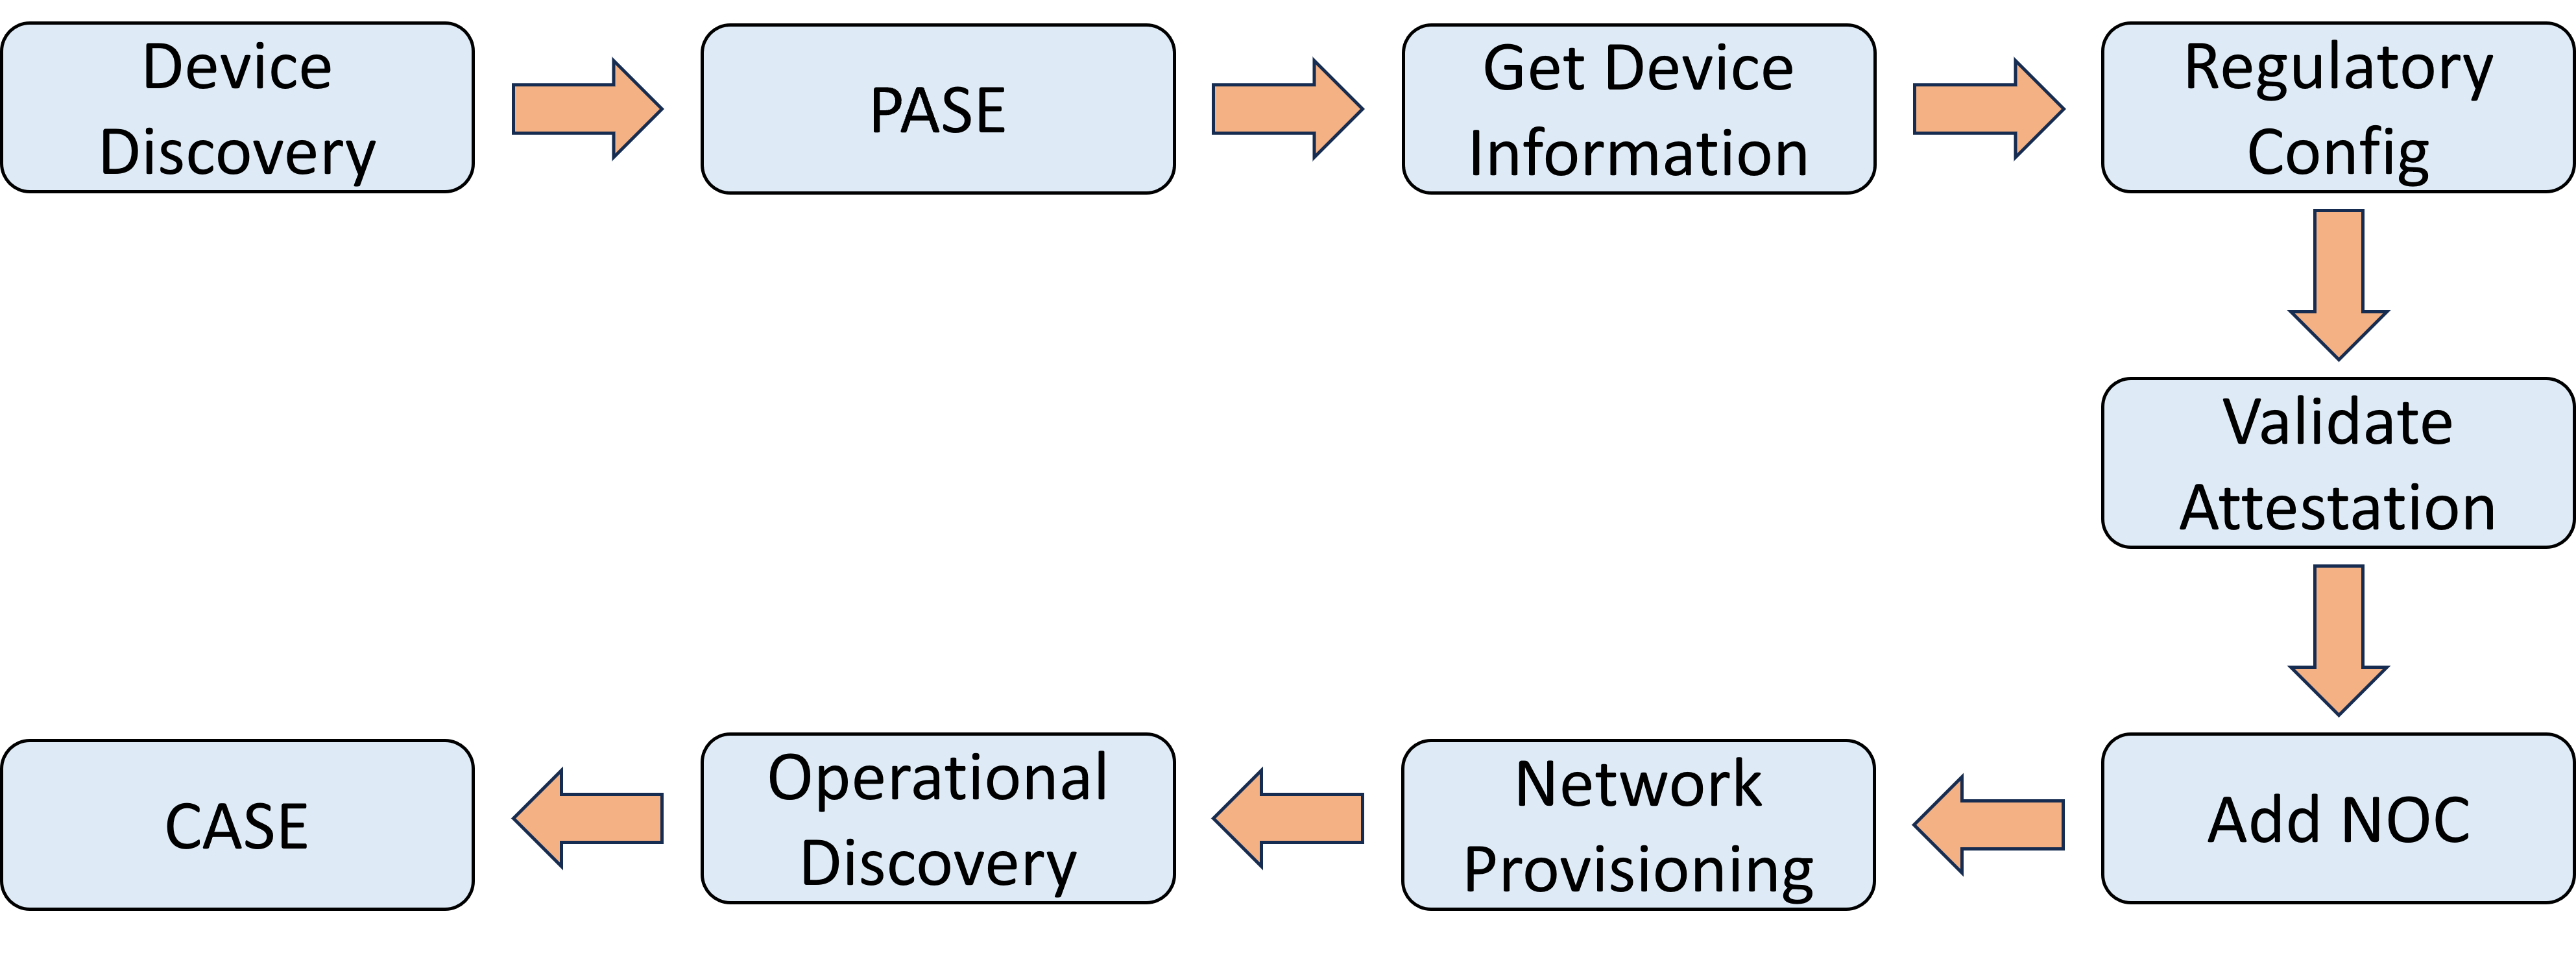
\includegraphics[scale=0.5]{com}
  \caption{Commissioning}
  \label{Commissioning}
\end{figure}
\begin{enumerate}
  \item Um mit dem Commissioning zu beginnen, muss sich der Commissionee bewerben. Die Bewerbung erfolgt über eine der drei Commissionable Discovery Methoden, die im nächsten Abschnitt erklärt sind.
  \item Nachdem der Commissioner die Bewerbung erkennt, verwendet er den Passcode aus dem Onboarding-Payload. PASE\footnote[8]{ Passcode Authenticated Session Establishment} ist eine Methode für die Einrichtung der Schlüssel und die Kommunikation. Der Commissioner richtet dabei fail-safe ein, was die Rückstellung des neuen Gerätes zu den Standardeinstellungen bei einem Fehler ermöglicht.
  \item Danach liest der Commissioner alle Informationen aus Cluster von Commissionee. 
  \item Mit ‚SetRegulatoryConfig‘ Command übergibt der Commissioner rechtliche Daten an Commissionee. Das kann Standort, Landeskode oder andere Standardisierungen sein.
  \item Um festzustellen, ob der Commissionee zertifiziert wurde und ein Matter-Gerät ist, wird die Attestation benötigt. Dabei zieht der Commissioner DAC\footnote[9]{Device Attestation Certificate}und PAI\footnote[10]{Product Attestation Intermediate } von Commissionee aus. Diese Zertifikate enthalten Vendor-ID, Produkt-ID und APK\footnote[11]{Attestation Public Key}. Nach Erhalt der Zertifikate stellt der Commissioner eine Anfrage, die mit APK unterschrieben werden soll und nutzt diese, um Authentizität von Commissionee zu bestätigen. Anschließend sendet der Commissioner eine CSR\footnote[12]{Certificate Signing Request} an dem Commissionee. Der Commissionee erstellt einen Schlüssel, der später bei CASE verwendet wird, und gibt die CSR an den Commissioner zurück.
  \item Der Commissioner verwendet Informationen aus CSR und übergibt diese an ADM\footnote[13]{ Administrative Domain Manager}, um einen NOC\footnote[14]{Node Operational Certificate} zu generieren. Zunächst installiert der Commissioner das Root-Zertifikat mit dem Kommando ‚AddTrustedRootCertReq‘ und anschließend das NOC mit dem Kommando ‚AddNOC‘.
  \item In diesem Schritt wird das Netzwerk für den Commissionee eingerichtet. Der Commissioner nutzt dabei folgende Befehle: ‚ScanNetworks‘, ‚AddOrUpdateWifiNetwork‘ und ‚ConnectNetwork‘. Wenn eine Ethernet-Verbindung besteht, entfällt dieser Schritt, da das Netzwerk bereits konfiguriert sein sollte. 
  \item Nachdem der Commissionee mit dem Netzwerk verbunden ist, sucht der Commissioner nach dem Gerät im Netzwerk und teilt anderen Geräten die IP-Adresse und Port des neuen Geräts.
  \item Der Commissioner initialisiert CASE\footnote[15]{ Certificate Authenticated Session Establishment}. Dabei tauschen der Commissioner und der Commissionee die Betriebszertifikate aus. Am Ende wird noch das Command ‚CommissioningComplete‘ gesendet und der fail-safe Timer wird automatisch gelöscht. Nach dem Commissioning ist das neue Gerät ein Node im Netzwerk
\end{enumerate}


\pagebreak

\listoffigures
\addcontentsline{toc}{chapter}{Abbildungsverzeichnis}

\end{document}